\documentclass{beamer}
\usetheme{Madrid}

\title{Conectando la Universidad de la Habana (UH)}
\subtitle{Asignatura: Diseño y Análisis de Algoritmos}
\author{Jabel Resendiz Aguirre \\ Noel Pérez Calvo \\ Arianne Camila Palancar Ochando}
\date{Enero 2026}

\begin{document}

\begin{frame}
  \titlepage
\end{frame}

\begin{frame}{Índice}
  \tableofcontents
\end{frame}

% Algoritmo Fuerza Bruta
\section{Algoritmo Fuerza Bruta}
\begin{frame}{Algoritmo Fuerza Bruta}
	\textbf{Idea principal:} Explorar todas las combinaciones posibles de aristas que puedan formar un árbol generador válido respetando los límites de grado.
	\vspace{0.3cm}
\begin{itemize}
  \item Generar todos los subconjuntos de $|V|-1$ aristas.
  \item Para cada subconjunto:
    \begin{itemize}
      \item Verificar si forma un árbol (conexo y acíclico)
      \item Comprobar que ningún vértice excede su límite de grado
      \item Calcular el costo total
    \end{itemize}
  \item Seleccionar la solución de menor costo
\end{itemize}

Por tanto, la complejidad temporal total del algoritmo es:
\[
\mathcal{O}\Bigg(\binom{m}{n-1} \cdot n\Bigg)
\]

\end{frame}

% Algoritmo Heurístico: Reducción del Árbol de Oportunidades
\section{Algoritmo Heurístico: Reducción del Árbol de Oportunidades}
\begin{frame}{Reducción del Árbol de Oportunidades}
  \textbf{Idea principal:} Aprovechar propiedades estructurales del árbol generador óptimo para reducir el grafo antes de construir la solución.
\begin{itemize}
  \item Se identifican aristas y vértices que necesariamente deben o no pueden estar en la solución óptima (lemas estructurales).
  \item Se eliminan aristas innecesarias y se fijan otras en la solución parcial.
  \item Esto reduce el tamaño del problema y acelera la construcción del árbol final.
\end{itemize}
	\textbf{Ejemplo de reducción:}
\begin{itemize}
  \item Toda arista incidente a un vértice hoja debe estar en la solución.
  \item Ninguna arista entre dos vértices de grado máximo 1 puede estar en la solución si $|V|>2$.
  \item Si un vértice $v$ de grado 2 conecta dos v\'ertices $u$ y $w$, si no existe un camino entre $u$ y $w$ que no pase por $v$ entonces tanto $\{u,v\}$ como $\{u,w\}$ deben pertenecer a la soluci\'on.
\end{itemize}
\end{frame}

\begin{frame}{Algoritmo y Complejidad}
	\textbf{Esquema del algoritmo:}
\begin{enumerate}
  \item Aplicar la reducción estructural al grafo ($O(n^3)$).
  \item Construir un árbol generador usando un algoritmo tipo Kruskal modificado para respetar los límites de grado.
  \item Mejorar la solución con técnicas de intercambio de aristas (1-opt y 2-opt).
\end{enumerate}
\vspace{0.2cm}
	\textbf{Complejidad:}
\begin{itemize}
  \item Reducción: $O(n^3)$
  \item Construcción inicial: $O(n)$
  \item 1-opt: $O(n)$, 2-opt: $O(n^2)$
  \item \textbf{Total:} $O(n^3)$
\end{itemize}
	\textbf{Ventaja:} Permite obtener soluciones de alta calidad en tiempo polinomial, viable para instancias grandes.
\end{frame}


\begin{frame}{Ejemplo}
\begin{columns}
    \column{0.5\textwidth}
        \centering
        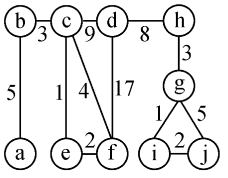
\includegraphics[width=0.9\textwidth]{1.png}
        \small{Figura 1: Grafo Original}
    \column{0.5\textwidth}
        \centering
        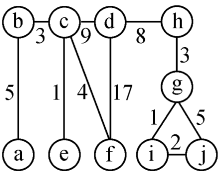
\includegraphics[width=0.9\textwidth]{2.png}
        \small{Figura 2: Grafo al quitarle la arista \{e,f\}}
\end{columns}
\end{frame}




\begin{frame}{Ejemplo}
\begin{columns}
    \column{0.5\textwidth}
        \centering
        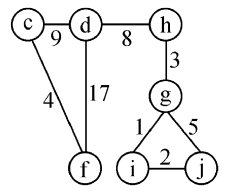
\includegraphics[width=0.9\textwidth]{3.png}
        \small{Figura 1: Grafo G}
    \column{0.5\textwidth}
        \centering
        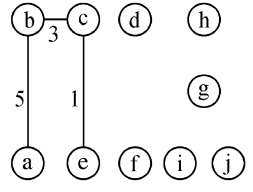
\includegraphics[width=0.9\textwidth]{4.png}
        \small{Figura 2: Grafo T*}
\end{columns}
\end{frame}


\begin{frame}{Ejemplo}
\begin{columns}
    \column{0.5\textwidth}
        \centering
        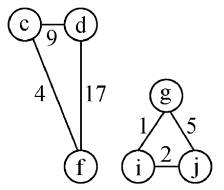
\includegraphics[width=0.9\textwidth]{5.png}
        \small{Figura 1: Grafo G  }
    \column{0.5\textwidth}
        \centering
        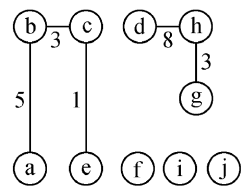
\includegraphics[width=0.9\textwidth]{6.png}
        \small{Figura 2: Grafo T*}
\end{columns}
\end{frame}



\begin{frame}{Ejemplo}
\begin{columns}
    \column{0.5\textwidth}
        \centering
        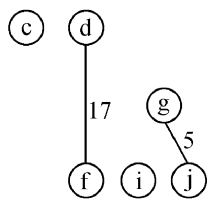
\includegraphics[width=0.9\textwidth]{7.png}
        \small{Figura 1: Grafo G }
    \column{0.5\textwidth}
        \centering
        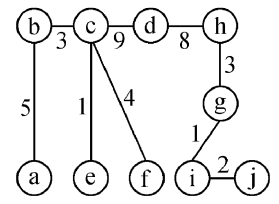
\includegraphics[width=0.9\textwidth]{8.png}
        \small{Figura 2: Grafo T*}
\end{columns}
\end{frame}


% Heurística Lagrangiana para DC-MST
\section{Heurística Lagrangiana para DC-MST}
\begin{frame}{Heurística Lagrangiana: Idea Principal}
\textbf{Idea principal:} Relajar las restricciones de grado usando multiplicadores Lagrangianos, transformando el problema en uno de árbol generador clásico con costos modificados.
\begin{itemize}
  \item Se obtiene una cota inferior resolviendo el MST con costos ajustados.
  \item Se usan multiplicadores para penalizar violaciones de grado y se actualizan con el método del subgradiente.
  \item Se construye una solución factible con un algoritmo tipo Kruskal modificado (KRUSKALX) y técnicas de mejora local.
\end{itemize}
\textbf{Componentes principales:}
\begin{enumerate}
  \item Relajación Lagrangiana y método del subgradiente
  \item Construcción heurística con prevención de infactibilidad
  \item Definición de problema restringido para acelerar el proceso
  \item Mejora local por intercambio de aristas
\end{enumerate}
\end{frame}

\begin{frame}{Heurística Lagrangiana: Esquema y Complejidad}
\textbf{Esquema del algoritmo:}
\begin{enumerate}
  \item Relajar restricciones de grado y resolver MST con costos modificados
  \item Actualizar multiplicadores Lagrangianos por subgradiente
  \item Construir solución factible con KRUSKALX y mejorarla localmente
  \item Repetir hasta convergencia o máximo de iteraciones
\end{enumerate}
\vspace{0.2cm}
\textbf{Complejidad:}
\begin{itemize}
  \item Por iteración: $O(n^2 m' + m' \log m')$, donde $m'$ es el número de aristas en el problema restringido
  \item Total: $O(K \cdot (n^2 m' + m' \log m'))$, con $K$ iteraciones
  \item Para grafos completos: $O(K n^3 \log n)$
\end{itemize}
\textbf{Ventajas:}
\begin{itemize}
  \item Proporciona cotas de calidad y soluciones factibles eficientes
  \item Escalable a instancias grandes (miles de vértices)
\end{itemize}
\end{frame}

% Implementación y Análisis Experimental
\section{Implementación y Análisis Experimental}
\begin{frame}{Resultados de Escalabilidad}
\textbf{Límite de Fuerza Bruta:} El algoritmo solo es viable hasta $n \approx 15$ vértices. Para $n=20$, el tiempo de ejecución excede los 61 segundos (timeout).

\vspace{0.3cm}
\textbf{Escalabilidad de las Heurísticas:}
\begin{itemize}
  \item \textbf{DCMST:} Escalable hasta $n \approx 960$ vértices (3.76 segundos). Falla en timeout para $n=1920$.
  \item \textbf{Lagrange:} Escalable hasta $n \approx 480$ vértices (0.86 segundos). Falla en timeout para $n=960$.
\end{itemize}

\vspace{0.3cm}
\textbf{Observaciones:}
\begin{itemize}
  \item DCMST muestra mejor escalabilidad práctica que Lagrange
  \item El comportamiento de DCMST se ajusta razonablemente a su complejidad teórica $O(n^3)$
  \item Lagrange presenta comportamiento más errático debido a la naturaleza iterativa del subgradiente
\end{itemize}
\end{frame}

\begin{frame}{Calidad de Soluciones}
\textbf{Evaluación sobre 100 instancias de prueba:}

\vspace{0.3cm}
\begin{table}
\centering
\begin{tabular}{|l|c|c|c|}
\hline
\textbf{Algoritmo} & \textbf{OK} & \textbf{FAIL} & \textbf{Resultado} \\
\hline
Brute Force & 100 & 0 & [OK] \\
DCMST & 95 & 5 & [FAIL] \\
Lagrange & 100 & 0 & [OK] \\
\hline
\end{tabular}
\end{table}

\vspace{0.3cm}
\textbf{Conclusiones:}
\begin{itemize}
  \item \textbf{Brute Force:} Garantiza optimalidad, pero solo viable para instancias pequeñas ($n \leq 15$)
  \item \textbf{DCMST:} Excelente escalabilidad y 95\% de exactitud, ideal para instancias grandes
  \item \textbf{Lagrange:} 100\% de exactitud con buena escalabilidad, mejor balance calidad-tiempo
\end{itemize}
\end{frame}

\end{document}
